\documentclass{article}
\usepackage{ctex}
\usepackage{graphicx}
\usepackage{amsmath}
\usepackage{indentfirst}
\usepackage{titlesec}
\usepackage{setspace}
\usepackage{subfigure}
\usepackage{caption}
\usepackage{float}
\usepackage{booktabs}
\usepackage{geometry}
\usepackage{multirow}
\geometry{left=2cm,right=2cm,top=2cm,bottom=2cm}
\title{\songti \zihao{2}\bfseries 闪锌矿晶体小论文}
\titleformat*{\section}{\songti\zihao{4}\bfseries}
\titleformat*{\subsection}{\songti\zihao{5}\bfseries}
\renewcommand\thesection{\arabic{section}}
\author{王启骅 PB20020580}
\begin{document}
	\maketitle
	\section{结构}
闪锌矿$ (ZnS) $结构如图1所示,S原子(绿色)位于$ 000,0\frac{1}{2}\frac{1}{2},\frac{1}{2}0\frac{1}{2},\frac{1}{2}\frac{1}{2}0 $,Zn原子(紫色)坐标$ \frac{1}{4}\frac{1}{4}\frac{1}{4},\frac{1}{4}\frac{3}{4}\frac{3}{4},\frac{3}{4}\frac{1}{4}\frac{3}{4},\frac{3}{4}\frac{3}{4}\frac{1}{4} $
\begin{figure}[!h]
	
	\centering
	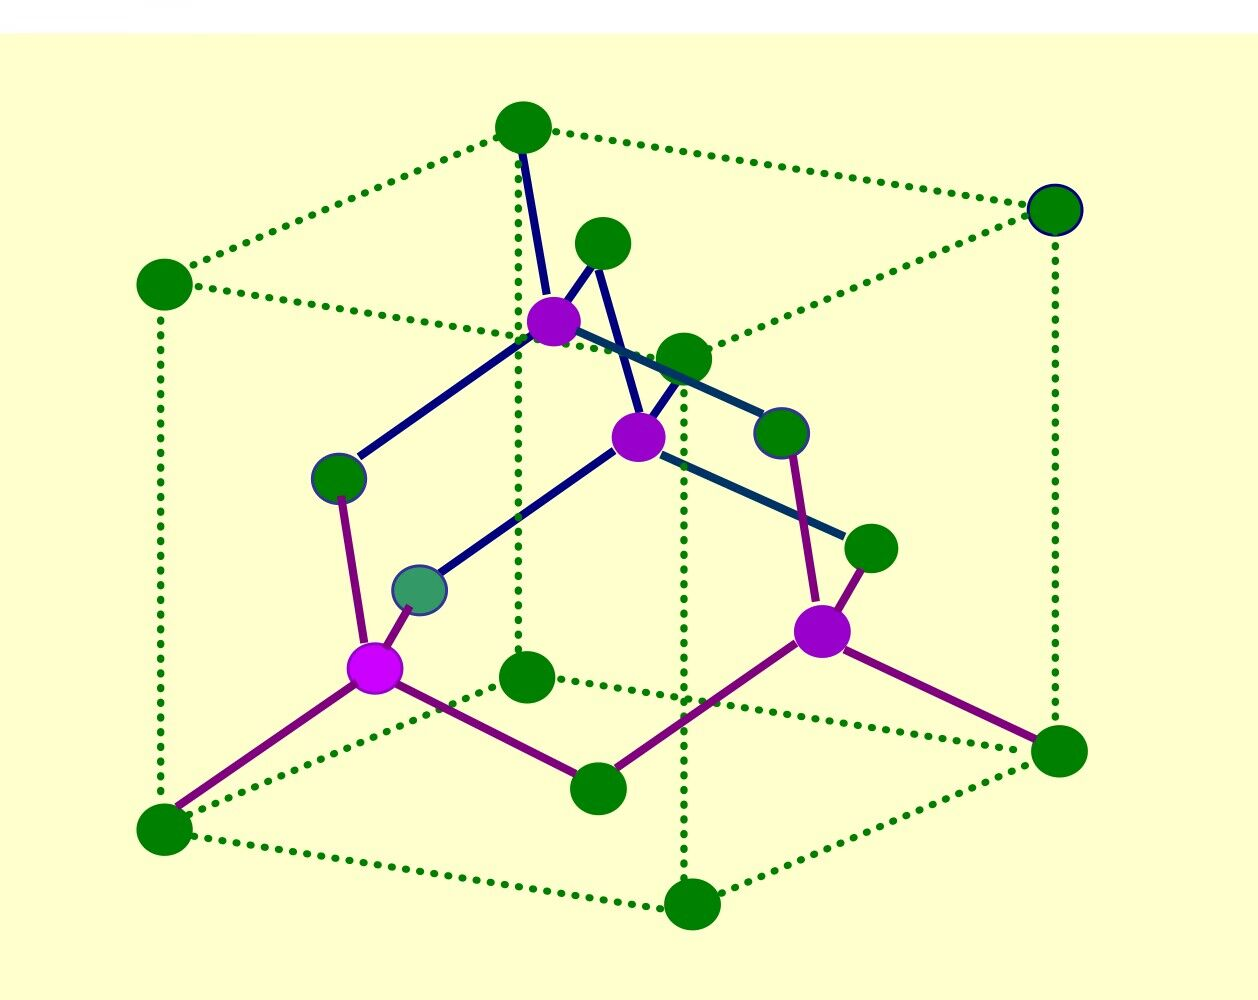
\includegraphics[scale=0.2]{结构}
	\captionsetup{font={small},labelfont=bf}
	\caption{\heiti\zihao{-5}闪锌矿结构}
	
\end{figure}


可以取如图2一个S原子连接四个Zn原子(由每个Zn与4个S相连,各占有$  \frac{1}{4} $)为一个基元,则可以等效于面心立方点阵。
\begin{figure}[!h]
	\centering
	\subfigure[基元]{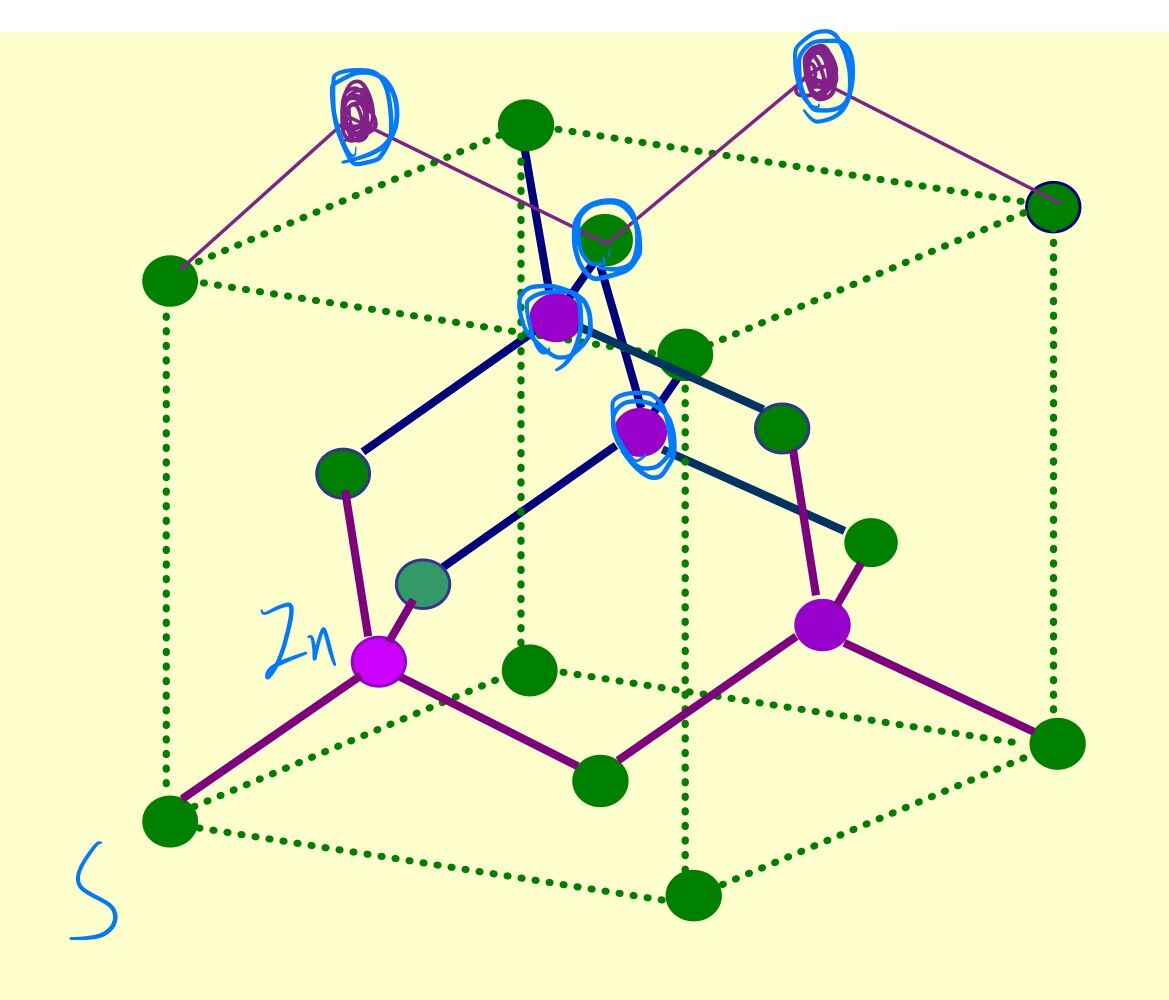
\includegraphics[scale=0.15]{基元}}
	\subfigure[等效面心立方晶格]{	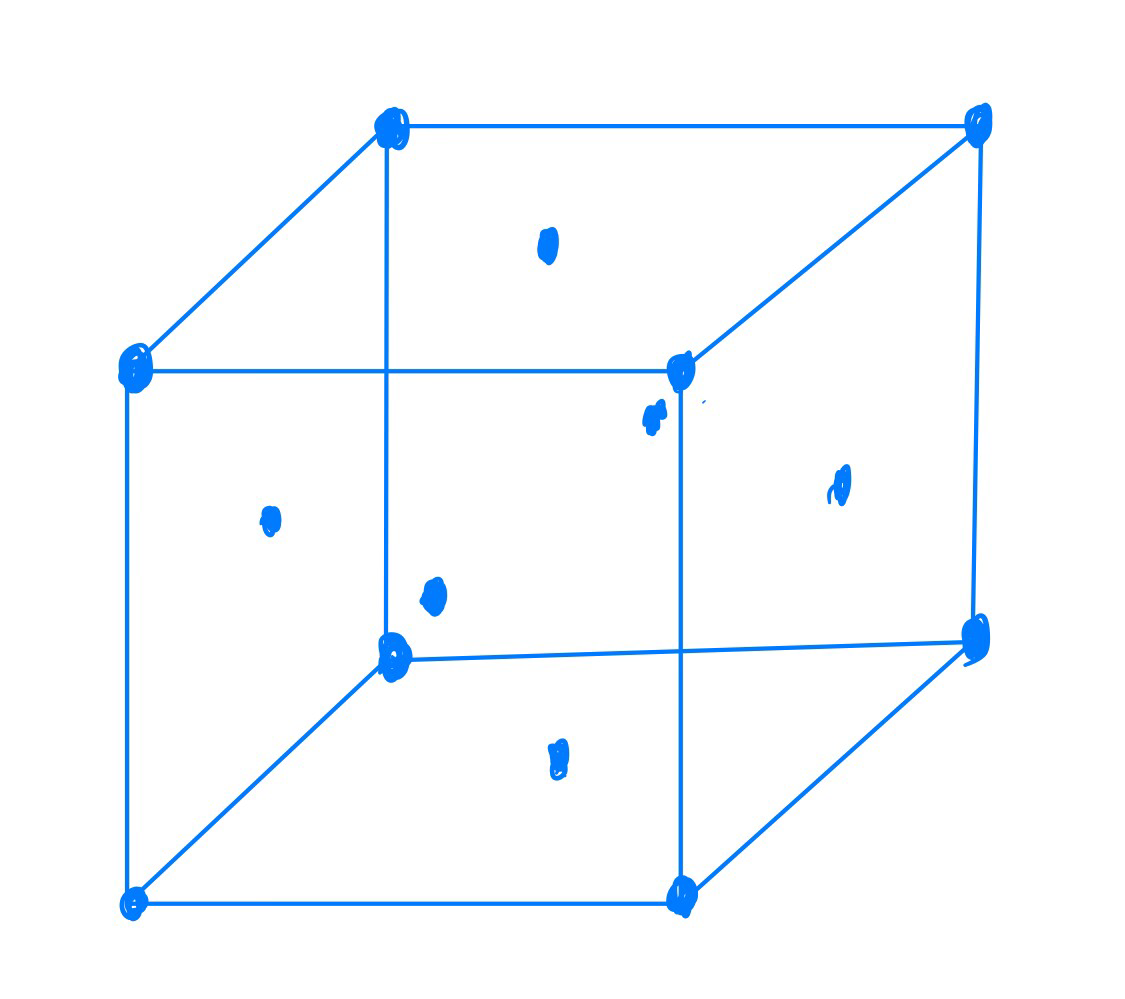
\includegraphics[scale=0.15]{面心}}
	\captionsetup{font={small},labelfont=bf}
	\caption{\heiti\zihao{-5}基元选取}
	
\end{figure}


闪锌矿的原胞如图3,连接顶点S原子到两个邻近的面心得到原胞基矢。
\begin{figure}[!h]
	
	\centering
	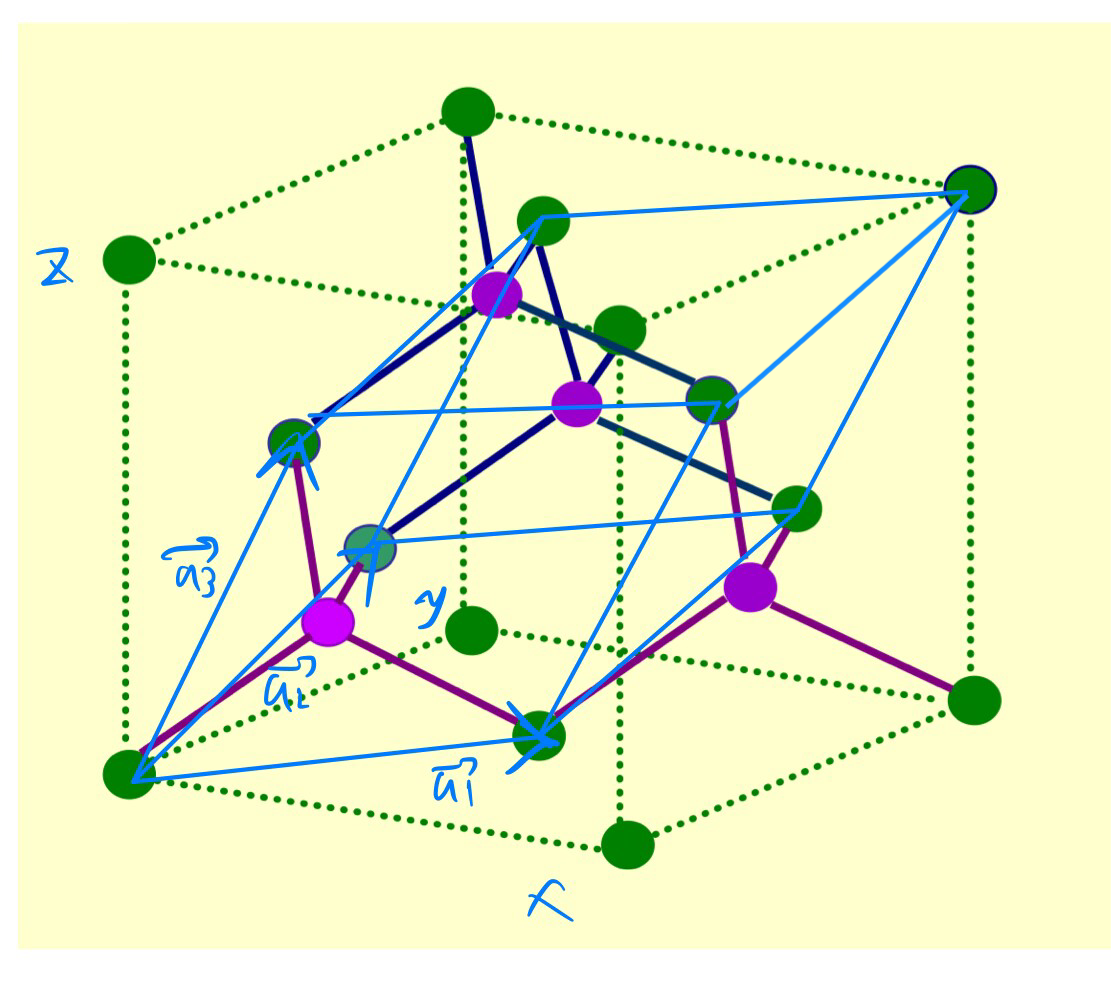
\includegraphics[scale=0.2]{原胞}
	\captionsetup{font={small},labelfont=bf}
	\caption{\heiti\zihao{-5}原胞}
	
\end{figure}
 \begin{equation}
	\begin{cases}
		\vec{\alpha_1}=\frac{a}{2}\hat{x}+\frac{a}{2}\hat{y}\\
		\vec{\alpha_2}=\frac{a}{2}\hat{x}+\frac{a}{2}\hat{z}\\
		\vec{\alpha_3}=\frac{a}{2}\hat{y}+\frac{a}{2}\hat{z}
	\end{cases}
\end{equation}


可见在一个原胞中,内部包含了一个Zn原子,其余的三个Zn原子在原胞外,且原胞八个顶点的S原子各占有$ \frac{1}{8} $,共有一个Zn,一个S。对应闪锌矿的化学组成ZnS。其Wigner-Seitz原胞对应于体心立方的布里渊区,即为正菱形十二面体。


	\section{对称性}
首先对面面心的连线为二重旋转轴,同时也为四重旋转反演轴,共3条;体对角线为三重旋转轴,共4条。


同时晶格表面的面对角线,与该面面心与对面面心连线轴构成的平面均为反映面,共有6个反映面。


闪锌矿由不同原子构成,其失去了金刚石原有的四度螺旋轴。
	
	\section{倒易点阵与布里渊区}
由于基元组成的晶格为面心立方,其倒易点阵为边长为$ \frac{4\pi}{a} $的体心立方。倒格子基矢
\begin{equation}
	\begin{cases}
		\vec{b_1}=\frac{2\pi}{a}(\hat{x}+\hat{y}-\hat{z})\\
		\vec{b_2}=\frac{2\pi}{a}(\hat{x}-\hat{y}+\hat{z})\\
		\vec{b_3}=\frac{2\pi}{a}(-\hat{x}+\hat{y}+\hat{z})
	\end{cases}
\end{equation}


对应的第一布里渊区为一个截角八面体如图4
\begin{figure}[!h]
	
	\centering
	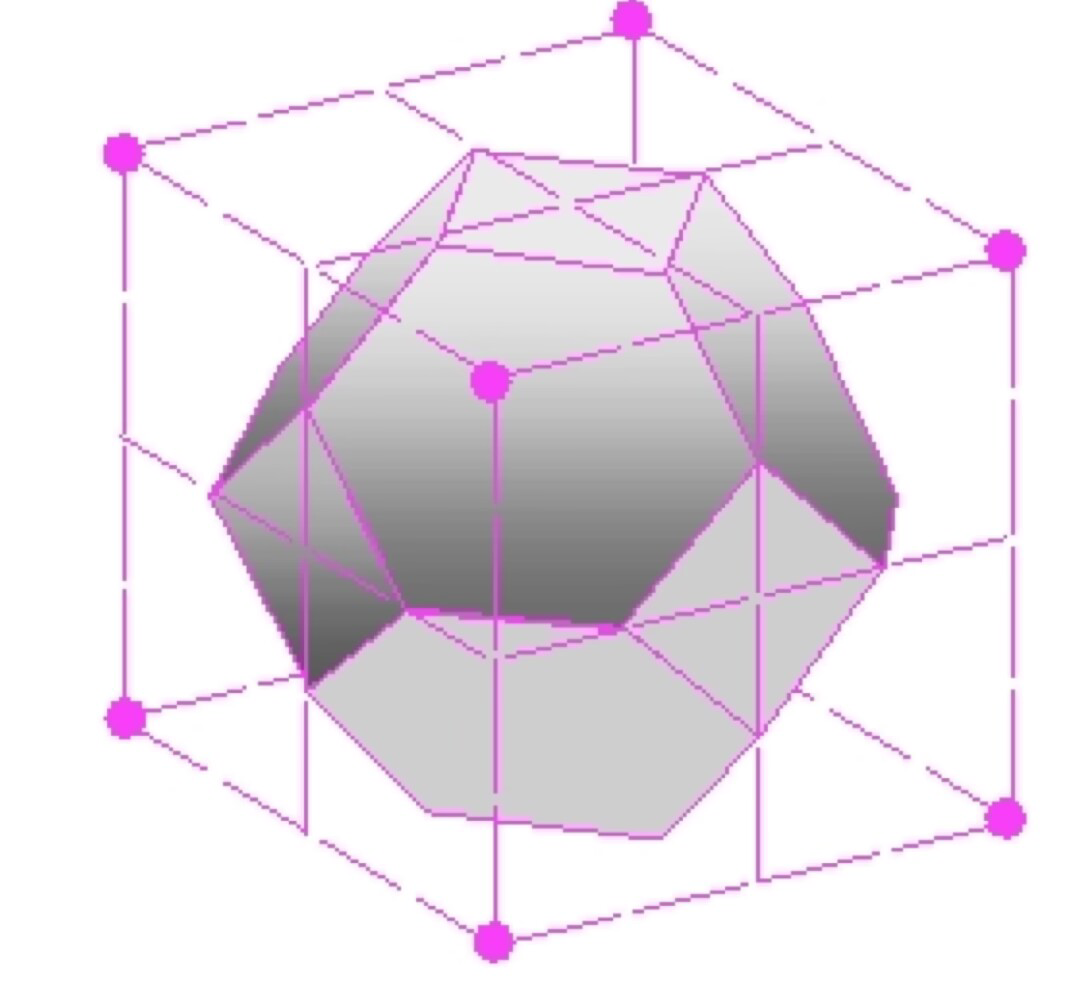
\includegraphics[scale=0.2]{布里渊区}
	\captionsetup{font={small},labelfont=bf}
	\caption{\heiti\zihao{-5}第一布里渊区}
	
\end{figure}


如图5进一步可以推知第二布里渊区为该体心立方本身(次近邻点为紫色,为近邻晶格的体心),第三布里渊区仍为截角八面体(第三近邻点为绿色,为对角晶格的体心)。
\begin{figure}[!h]
	
	\centering
	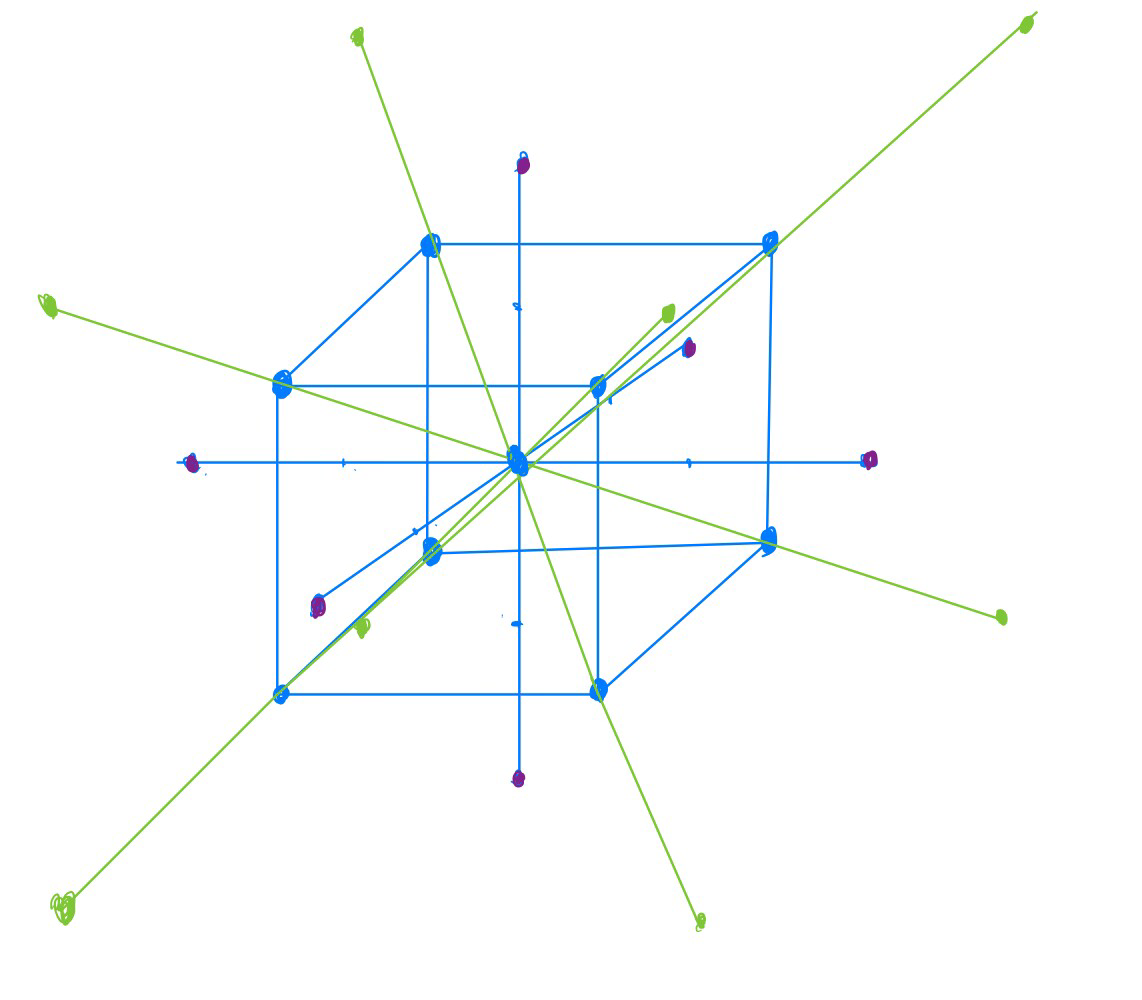
\includegraphics[scale=0.2]{高}
	\captionsetup{font={small},labelfont=bf}
	\caption{\heiti\zihao{-5}第2、3布里渊区}
	
\end{figure}
	\section{总结}
本文讨论了有关闪锌矿晶体的结构、原胞、对称性、倒易点阵、布里渊区等特点与性质。实际上闪锌矿结构与金刚石类似,主要是基元变为ZnS,导致对称性有一定降低。
\end{document}